%%%%%%%%%%%%%%%%%%%%%%%%%%%%%%%%%%%%%%%%%%%%%%%%%%%%%%%%%%%%%%%%%%%%%%%
% Prompts Are Advisory, Verification Is Enforcement
% IEEE Transactions on Software Engineering submission.
%
% This is the two-column condensation of the sn-jnl manuscript in
% ../emse_latex/. Every number is the same; what moved is prose, three
% tables and one proof, all of which are in the appendix or the
% replication package. See CUTS.md for what was removed and where it went.
%%%%%%%%%%%%%%%%%%%%%%%%%%%%%%%%%%%%%%%%%%%%%%%%%%%%%%%%%%%%%%%%%%%%%%%
\documentclass[journal]{IEEEtran}

\usepackage{amsmath,amssymb,amsthm}
\usepackage{booktabs}
\usepackage{graphicx}
\usepackage[hidelinks]{hyperref}
\usepackage{url}
\usepackage{balance}
\usepackage{microtype}
\usepackage[htt]{hyphenat}   % let long \texttt rule names break
\tolerance=1200
\emergencystretch=1.5em

% Eleven floats in fourteen pages. The stock parameters queue them until a page
% top can take them all, which put four on one page with the text in fragments.
\renewcommand{\topfraction}{0.9}
\renewcommand{\bottomfraction}{0.6}
\renewcommand{\textfraction}{0.08}
\renewcommand{\floatpagefraction}{0.75}
\renewcommand{\dbltopfraction}{0.9}
\renewcommand{\dblfloatpagefraction}{0.75}
\setcounter{topnumber}{3}
\setcounter{bottomnumber}{2}
\setcounter{totalnumber}{4}

\newtheorem{definitionx}{Definition}
\newtheorem{proposition}{Proposition}

\hyphenation{mlcompass evi-dence-closed}

\begin{document}

\title{Prompts Are Advisory, Verification Is Enforcement:\\
An Evidence-Bound Runtime Contract for\\
LLM Narration of Pipeline Evidence}

\author{Hakan~Sabuni\c{s},
        Yusuf~\"Unl\"u,
        and~Mehmet~Kemal~\"Ozdemir% <-this % stops a space
\thanks{The authors are with the School of Engineering and Natural Sciences,
Istanbul Medipol University, Istanbul, T\"urkiye.
E-mail: hakan.sabunis@std.medipol.edu.tr}}

\markboth{IEEE Transactions on Software Engineering}%
{Sabuni\c{s} \MakeLowercase{\textit{et al.}}: Prompts Are Advisory, Verification Is Enforcement}

\IEEEtitleabstractindextext{%
\begin{abstract}
Software tools increasingly place a large language model between a
deterministic analysis and the engineer who acts on it; when the explanation
cites a column, defect or number the analysis never produced, the engineer acts
on something never observed. We identify \emph{evidence-closed} narration
tasks, whose citable entities and checkable quantities are finite and
machine-enumerable at the moment of the call, which makes faithfulness
decidable on the structured claim channels. A two-tier \emph{evidence-bound
runtime contract} built on that property ships in the narration path of
\textbf{mlcompass}, an open-source ML-pipeline assistant: Tier~A binds
field-indexed admissible sets into the tool schema at call time, and Tier~B
re-verifies the returned payload in host code. Over 3,800 live responses and
175 scored runs, the dominant failure is not invention but \emph{misfiling} ---
a real evidence item placed where it is not admissible: 162 of 162 flagged
entities on a data-leakage task, and 11 of 12 wrong values on a
dataset-profiling task. Inside one guardrail toolkit, with loop, budget, prompt
and model held fixed, the stock validator leaves 35.0\,\% of responses with a
structured-evidence violation; our validator, and equally the toolkit's own
choice check once its list is bound to the evidence, leaves none observed in
200 responses, bounding the true rate below 1.9\,\% at 95\,\% confidence. On an
enforced arm that absence is a property of the verifier; what the sample
measures is its cost: every violation was repaired by a corrective retry, and
binding the schema removes retries only on the channel an enum can express.
The unconstrained rate is unstable: three runs of one model name over nine days
move the toolkit default from 35.0\,\% to 47.5\,\%. Downstream, an arm given
only the names of the scored rules beats the arm given the tool's real
findings, and we withdraw an earlier causal attribution. The guarantee covers
the structured channels only; measuring the free-text narration finds no
content displaced into it by enforcement.
\end{abstract}

\begin{IEEEkeywords}
Large language models, faithfulness, runtime verification, structured
output, constrained generation, data leakage.
\end{IEEEkeywords}}

\maketitle
\IEEEdisplaynontitleabstractindextext
\IEEEpeerreviewmaketitle

%%%%%%%%%%%%%%%%%%%%%%%%%%%%%%%%%%%%%%%%%%%%%%%%%%%%%%%%%%%%%%%%%%%%%%%
\section{Introduction}\label{sec:intro}
%%%%%%%%%%%%%%%%%%%%%%%%%%%%%%%%%%%%%%%%%%%%%%%%%%%%%%%%%%%%%%%%%%%%%%%

\IEEEPARstart{M}{achine-learning} practice runs on single-purpose tools ---
profilers~\cite{ydata}, experiment trackers~\cite{mlflow,tensorflow}, automated
model search~\cite{autosklearn} --- and none tells the engineer what the
results \emph{mean}. The now-standard answer is agentic: an LLM calls the
tools, reads their structured output and explains
it~\cite{react,toolformer,mcp}. LLMs are known to produce content their input
does not support~\cite{ji,huang}, and assistants built on them still fail real
software tasks at substantial rates~\cite{codex,swebench}.

In an advisory ML setting the narrated object is \emph{structured evidence} ---
facts a deterministic tool actually measured --- and a structured claim about
it can be wrong in two ways. It can \emph{invent}: name an entity or quote a
quantity that appears nowhere in the evidence. Or it can \emph{misfile}: put
something the evidence really contains where it is not admissible --- a
metric's name in a column field, one column's measurement attributed to
another. The literature studies the first as hallucination. On both tasks in
this paper the second dominates: 162 of 162 flagged entities on the first were
misfiled and none invented, and 11 of 12 wrong values on the second were real
measurements of a different column. We therefore reserve
\emph{hallucination} for invention. Misfiling is the more dangerous for a
reader, because every name and number in a misfiled claim is one the tool
really produced, and a wrong diagnosis delivered fluently is acted on.

This paper is built on one observation: what the narrator may cite is
\emph{finite and machine-enumerable at the moment of the call}.

\begin{definitionx}[Evidence-closed narration]\label{def:closed}
A narration task is \emph{evidence-closed} if the set of citable entities and
verifiable quantities is finite and machine-enumerable at the moment of the
narration call.
\end{definitionx}

Once a task is evidence-closed, faithfulness \emph{on its structured claim
channels} stops being a modelling problem: entity citations become membership
tests against the domain admissible for their field, quantitative claims become
numeric comparisons, and coverage of the critical finding is one more
membership test. The sensible goal changes from \emph{mitigation} to
\emph{prevention}. The narrowing matters and we hold to it: a free-text
sentence can name only real columns, quote only real values, and still assert
a causal story the evidence does not support.

Constrained decoding~\cite{outlines,lmql,gcd,guidance} needs the token
distribution, which commercial APIs do not expose, and a per-call JSON
schema~\cite{structured} helps only if the provider's enforcement is trusted,
which for a safety claim it should not be. Our answer is a two-tier
\textbf{evidence-bound runtime contract}. \emph{Tier~A} generates the
\texttt{enum} domains of the narrator's tool-input fields from the evidence at
call time. \emph{Tier~B} re-checks the returned answer in plain code ---
entity soundness, value soundness of \{column, statistic, value\} claims, and
completeness with respect to the top-ranked candidate --- with corrective
retry, residual stripping and omission flagging. It is the default narration
path of \textbf{mlcompass}, an open-source (MIT) ML-pipeline assistant,
guarding the investigation that fires when a metric looks too good to be true
($R^2>0.999$ or $\mathrm{AUC}>0.995$, motivated by the leakage problem of
Kaufman \emph{et al.}~\cite{leakage}). We say \emph{shipped}, not
\emph{production}: we have no deployment telemetry.

\textbf{What survives.} Two claims were withdrawn after arms we ran to attack
them succeeded: one about \emph{whose} validator does the work
(Section~\ref{sec:rq3}) and a causal one about downstream code quality
(Section~\ref{sec:rq5-rubric}). Neither touches this: \emph{for a narration
task whose citable entities and checkable quantities are finite and enumerable
at the moment of the call, faithfulness on the structured claim channels is
enforceable by construction, in plain host code, behind a commercial API that
exposes no logits} --- provided the admissible set is computed from the
evidence at call time and checked where we control the check. We also report
eleven faults in our own instruments in the body
(Section~\ref{sec:instruments}): a defect found by the authors is evidence
about the instrument, and one found by a reader is evidence about the authors.

We ask \textbf{RQ1} how an unconstrained narrator of evidence-closed material
fails, and whether the failure matches the literature's name for it;
\textbf{RQ2} whether the contract prevents it on the validated channels;
\textbf{RQ3} how it compares with the structured-output and validate-and-retry
alternatives a practitioner would reach for; \textbf{RQ4} how far wording alone
moves compliance; \textbf{RQ5} whether deterministic findings reduce predefined
defect classes in the code a model writes; and \textbf{RQ6} whether the
contract transposes to a second evidence shape.

We contribute: (i) \textbf{the evidence-closed class} and a contract over it
(Definitions~\ref{def:closed} and~\ref{def:contract}) whose admissible domains
are \emph{indexed by field and derived from the evidence at call time}, which
is what separates misfiling from invention and lets a generic check enforce it;
(ii) \textbf{a controlled validator swap inside a released guardrail toolkit}:
with reask loop, budget, prompt and model fixed, Guardrails~AI's default leaves
35.0\,\% of responses with a violation and our validators leave none observed
in 200 --- but so does the toolkit's \emph{own} acceptable-values check with
its list built from $E$ at call time, so the binding does the work, not our
validator; (iii) \textbf{a decomposition} of the failure into invented and
misfiled entities; (iv) \textbf{a pre-registered downstream benchmark}, 175
scored runs over four models and three datasets, whose two added arms each
attack our own attribution; and (v) \textbf{a replication package} with every
emitted script, every model reply, one record per live response, the frozen
protocols, the amendment log and the instrument faults.

%%%%%%%%%%%%%%%%%%%%%%%%%%%%%%%%%%%%%%%%%%%%%%%%%%%%%%%%%%%%%%%%%%%%%%%
\section{Background and Related Work}\label{sec:related}
%%%%%%%%%%%%%%%%%%%%%%%%%%%%%%%%%%%%%%%%%%%%%%%%%%%%%%%%%%%%%%%%%%%%%%%

\subsection{Faithfulness, tool use and constrained generation}

Ji \emph{et al.}~\cite{ji} and Huang \emph{et al.}~\cite{huang} survey
hallucination; the failure we target is extrinsic in their taxonomy, but with
structure the general problem lacks: the source is a finite dictionary, so the
check is decidable. Xu~\cite{xu2025openworld} argues hallucination is
unavoidable in an open world while a closed world admits mitigation;
evidence-closed narration is a shipped closed world in which the mitigable case
is eliminated on the verified channels. Luo \emph{et al.}~\cite{luo2026removal}
use the same soundness and incompleteness vocabulary for a model's own
explanations, where the object is the model's reasoning and the intervention is
on the input. Data-to-text work scores generated text against a
table~\cite{dhingra2019parent,maynez2020faithfulness}; what it lacks is a
producer small enough to enumerate and pin into the call.

ReAct~\cite{react}, Toolformer~\cite{toolformer} and tool-integration
standards~\cite{mcp} govern how an agent \emph{acts}, not what it may
afterwards \emph{say} about a tool's output. Provenance surveys reconstruct
evidence support from traces after the fact~\cite{wang2026agenttraces}; Ng
\emph{et al.}~\cite{ng2026runtimecontract} argue independently that agent
safety belongs in a runtime contract. We instantiate one at that boundary.

Outlines~\cite{outlines}, LMQL~\cite{lmql}, grammar-constrained
decoding~\cite{gcd} and Guidance~\cite{guidance} constrain decoding, and
provider APIs validate tool calls against a declared schema~\cite{structured}.
Varying a constraint with the input is not new: \cite{gcd} does it, and
CHyD~\cite{signe2026chyd} restricts generation to spans present in the
retrieved context --- but needs logit access, which a commercial endpoint
withholds. What differs here is what the domain is bound to, \emph{when}, and
who enforces it: a deterministic producer's output, bound at call time rather
than at curation time~\cite{ren2026egvar} or decode time, and enforced in host
code.

\subsection{Where the enforcement lives}\label{sec:taxonomy}

\begin{table}[t]
\caption{Where enforcement lives. Only the last three rows are available behind
a commercial endpoint, and only the last binds its admissible set to the
evidence at the moment of the call.}
\label{tab:taxonomy}
\centering
\footnotesize
\setlength{\tabcolsep}{3.4pt}
\begin{tabular}{@{}llll@{}}
\toprule
Position & Needs & Guarantees & Example \\
\midrule
Decode, token & logits & grammaticality & \cite{outlines, gcd} \\
Decode, closed loop & logits & --- (empirical) & \cite{cruz2026atlasrtc} \\
Decode, span & logits & verbatim spans & \cite{signe2026chyd} \\
Provider schema & --- & structure, uncertifiable & \cite{structured} \\
Code, author-time & --- & policy contracts & \cite{ahn2026harness} \\
Code, accumulated & --- & per-claim provenance & \cite{du2026ledgermind} \\
\textbf{Code, call-time} & \textbf{---} & \textbf{faithfulness to $E$}
  & \textbf{here} \\
\bottomrule
\end{tabular}
\end{table}

Table~\ref{tab:taxonomy} locates this paper by where the thing that cannot be
talked out of its job sits. The logit-level rows are stronger than anything we
do and unavailable behind the endpoints we target.
ATLAS-RTC~\cite{cruz2026atlasrtc} intervenes during decoding with masking and
rollback, gaining 20--37.8 points of first-attempt success; its finding that
many failures are decoding artefacts is the most plausible mechanism we know
for our paraphrase sweep. Life-Harness~\cite{xu2026lifeharness} improves 116 of
126 settings by evolving the harness alone, empirically rather than by
guarantee, and Le~\cite{le2026schemakey} shows schema-key wording moves
accuracy in both directions --- a reason to distrust an uncertified schema
(Section~\ref{sec:rq3-degenerate}).

\textbf{Closest in design.} Ahn and Kim~\cite{ahn2026harness} run our
experimental design on a policy contract --- determinism in code, model fixed,
enforcement layer varied --- and find what we find: prompts let violations
through, a bolt-on guardrail over-refuses (88/120 utility against 120/120), and
only code-owned enforcement keeps both, over 270 runs on three hosted models.
Their contract is fixed when the harness is written; ours has no admissible
domain until the evidence exists. An author-time contract cannot say ``cite
only these ten column names''.

\textbf{Closest in mechanism.} LedgerMind~\cite{du2026ledgermind} lets claims
cite only active ledger entries, checks entity and numeric grounding, and
restricts repair to transitions that cannot add content without provenance.
Three of those are our Tier~B channels and the fourth is our repair asymmetry
(Proposition~\ref{prop:asym}); we derived it independently and claim no
priority. Their ledger accumulates, so the admissible set moves; ours is
complete before the call, which is what lets the domain go into the schema as
an enum.

\textbf{Closest in domain.} EviBound~\cite{chen2025evibound} governs an ML
research agent with an approval gate on acceptance-criteria schemas and a
verification gate that queries MLflow for a run, its artifacts and a terminal
status, optionally checking named metric values, with bounded retries; it
reports 0\,\% hallucination on eight tasks, eleven months before our
measurements. The two-gate shape, bounded retry and deterministic post-check
are shared. EviBound verifies that a claimed \emph{action} occurred; we verify
what may be \emph{said} about a measurement already taken, and bind that domain
into the call's schema before the model writes.

%%%%%%%%%%%%%%%%%%%%%%%%%%%%%%%%%%%%%%%%%%%%%%%%%%%%%%%%%%%%%%%%%%%%%%%
\section{Evidence-Closed Narration}\label{sec:theory}
%%%%%%%%%%%%%%%%%%%%%%%%%%%%%%%%%%%%%%%%%%%%%%%%%%%%%%%%%%%%%%%%%%%%%%%

\subsection{The evidence, and why admissibility is per field}

In the leakage investigation this paper studies, the deterministic layer
produces an evidence dictionary $E$: the suspicious metric and its value;
per-feature correlations against the target $y$ --- whichever of $\rho_P$ and
$\rho_S$ has the larger magnitude, sign preserved; a ranked candidate-leak set
$C=\{c:\max(|\rho_P(c,y)|,|\rho_S(c,y)|)\ge 0.99\}$; and the perfect-match rate
$P(\hat y=y)$. Spearman is there because monotone target transforms pull
$\rho_P$ down while $\rho_S$ stays at 1: our log-target leak sits at
$\rho_P=0.93$ against $\rho_S=0.999$ and would slide under a Pearson-only
filter.

A single entity universe $A_E$ --- every string the evidence mentions --- is
the obvious formalisation and the wrong one: under it, a \texttt{column} field
reading \texttt{r2} is sound, because \texttt{r2} is in the evidence as the
name of the \emph{metric}. Section~\ref{sec:rq1} shows this case, not
invention, is what the unconstrained narrator does. We therefore index
admissibility by field. For the schema's reference-bearing fields $F$ --- in
the leakage contract \texttt{columns\_referenced}, \texttt{claims[].column} and
\texttt{claims[].statistic} --- $A_{E,f}\subseteq A_E$ with
$A_E=\bigcup_{f\in F}A_{E,f}$, and the column and statistic domains are
disjoint. A token is \emph{misfiled} when it is in $A_E$ but not in $A_{E,f}$
for its field $f$, and \emph{invented} when it is in neither. Tier~A binds
$A_{E,f}$, not $A_E$, into each field's enum.

\subsection{The contract, stated as an invariant}

\begin{definitionx}[Evidence-bound runtime contract]\label{def:contract}
Let $E$ define field-indexed admissible sets $\{A_{E,f}\}_{f\in F}$, a value
table $V_E$ over (entity, statistic) pairs, a tolerance $\tau$, and an anchor
$a^*$. A structured response $r$ \emph{satisfies} the contract
$\mathcal{C}_E$ if
\textbf{(C1)} every token $x$ that $r$ places in a field $f \in F$ has
$x \in A_{E,f}$;
\textbf{(C2)} every structured claim $(e,s,v)$ in $r$ has
$(e,s) \in \mathrm{dom}(V_E)$ and $|v - V_E(e,s)| \le \tau$; and
\textbf{(C3)} if $r$ commits to a verdict, $a^*$ is among the entities $r$
references.
\end{definitionx}

Tier~B enforces (C1) and (C2) on the structured channels it returns: a response
violating either is sent back, at most twice, with the violation named, and
whatever still violates it is deleted. Hence \emph{no structured claim that
Tier~B returns violates (C1) or (C2)}. That is a property of the verifier,
established by construction and pinned by offline mutation tests
(Section~\ref{sec:rq3}), not an empirical rate; what a battery measures on an
enforced arm is how often the verifier acted and what that cost
(Table~\ref{tab:retry}). We report a clean enforced arm as \emph{none observed
in $N$} with its interval, never as a rate of zero. (C3) cannot be enforced
the same way.

\begin{proposition}[Repair asymmetry]\label{prop:asym}
Soundness is safe-repairable by deletion: the projection $\Pi_E(r)$ removing
every violating element is sound, idempotent, and the identity on sound
responses. Completeness is not: any repair must add a reference the model did
not produce.
\end{proposition}

\begin{IEEEproof}[Proof sketch]
Deletion preserves membership and tolerance and can remove every violating
element. For completeness, deleting the verdict would discharge the
obligation, but the schema requires \texttt{verdict}, and substituting
\texttt{cannot\_determine} would attribute to the narrator a stance it did not
take; both premises are stipulations of this contract, not facts about
narration. Given them, every remaining repair inserts an anchor reference
absent from $r$.
\end{IEEEproof}

So Tier~B strips unsound content and only \emph{flags} a persistent omission.
This is a monotonicity argument, not the safety/liveness result it
resembles~\cite{schneider2000enforceable,alpern1985liveness}, and it runs
opposite to the security case: over a narrator, insertion is inadmissible,
because an inserted reference fabricates attribution rather than correcting an
action.

\begin{proposition}[Linear-time verification]\label{prop:linear}
With $m=\sum_f|A_{E,f}|$, deciding (C1)--(C3) for a structured response $r$
takes $O(|r|)$ expected time after $O(m+|V_E|)$ preprocessing.
\end{proposition}

\begin{IEEEproof}
Hash each $A_{E,f}$ and $V_E$ once; each entity, claim and anchor check is then
one hashed lookup with keys of bounded length.
\end{IEEEproof}

The proposition is a feasibility property, not a contribution. What is not
shallow is the indexing: an earlier version of our own scorer keyed $V_E$ on
the column alone and compared every claim against that column's correlation,
whatever statistic it named (Section~\ref{sec:instruments}).

%%%%%%%%%%%%%%%%%%%%%%%%%%%%%%%%%%%%%%%%%%%%%%%%%%%%%%%%%%%%%%%%%%%%%%%
\section{The Artifact}\label{sec:contract}
%%%%%%%%%%%%%%%%%%%%%%%%%%%%%%%%%%%%%%%%%%%%%%%%%%%%%%%%%%%%%%%%%%%%%%%

\begin{figure}[t]
\centering
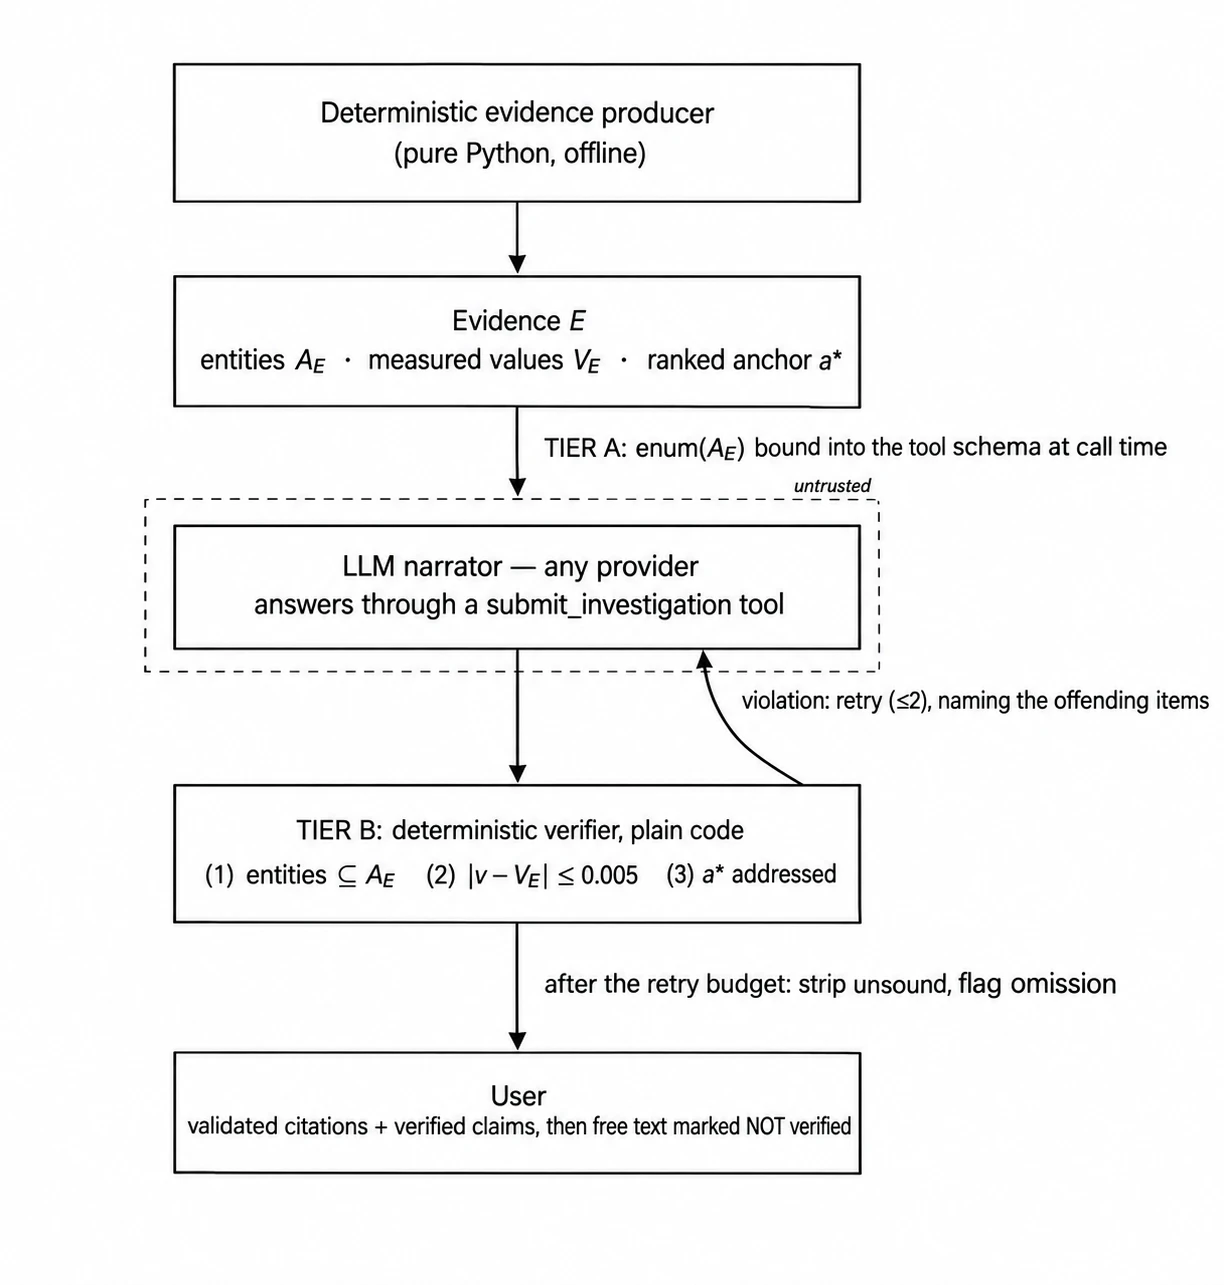
\includegraphics[width=\columnwidth]{fig1_contract.png}
\caption{The evidence-bound contract. Tier~A binds the tool schema's enums to
$E$ at call time; Tier~B re-checks the returned answer in host code, retries
with the offending items named, and after the budget strips unsound content
and flags a persistent omission. The dashed boundary encloses the narrator
alone. The producer is trusted, not verified; the free-text field reaches the
user marked unverified; and the response is guaranteed consistent with $E$, not
$E$ with the world.}
\label{fig:contract}
\end{figure}

\subsection{Architecture and the trust boundary}

Figure~\ref{fig:contract} splits the system at a trust boundary. On one side is
everything deterministic: the pure-Python evidence producer, $E$, the Tier~B
verifier and the user-facing output; on the other, the LLM narrator, untrusted
whoever serves it. The system has three \emph{layers} --- evidence production;
a narrator told the rules in words (Section~\ref{sec:rq4} measures what that is
worth); and the evidence-bound schema, through whose
\texttt{submit\_investigation} tool answers arrive --- and the contract spans
the last two as two enforcement \emph{tiers}. \textbf{Tier~A} restricts
\texttt{columns\_referenced} and \texttt{claims[].column} by \texttt{enum}s
built from $E$ at call time. \textbf{Tier~B} re-checks the returned tool input
in plain code for \emph{entity soundness} (C1), \emph{value soundness} within
$\tau=0.005$ (C2), and \emph{completeness}: a verdict other than
\texttt{cannot\_determine} must address the top-ranked candidate (C3).

A failed check earns a corrective retry naming the offending items (budget 2).
Whatever is still unsound is stripped, a persistent omission is flagged, and
completeness is re-checked after stripping, because deleting an unsound claim
can orphan the anchor. Every other failure closes the same way: a missing tool
call or required field is retried and then aborted, leaving the deterministic
evidence panel --- printed unconditionally --- as all the user sees, and a
provider exception propagates rather than degrading. No unvalidated structured
claim is reachable through any path.

\subsection{One contract, two instances}\label{sec:generic}

For most of this study the code was an instance: one column set,
\texttt{claims[].statistic} frozen to a one-element enum, and a claim checked by
looking its column up in the correlation map. The contract is now a layer: a
spec says how to read one evidence shape, binding yields the field-indexed
domains, value table and anchor, and the verifier, stripper, retry text and
schema builder name no task. Leakage is one spec of about forty lines; a
dataset profiler is a second, with every column of the frame admissible,
thirteen statistics per column, and a statistic set computed per call because
a categorical column carries a cardinality and no mean.

Extraction exposed what one task could not: \textbf{the value table must be
keyed on $(\text{entity}, \text{statistic})$}. With one statistic per column
the two keyings coincide; in a profile, \texttt{age.mean} is $38.5$ and
\texttt{age.missing\_pct} is $0.012$, and an entity-keyed table checks a claim
about one against the other --- the scorer defect of
Section~\ref{sec:instruments}, reappearing in the production path. And the
evidence's surface shape must match the flat claim slot: narrators handed a
nested quantity invent a flattening, and they invented five.

\subsection{What the invariant does not cover}

\emph{Within the validated channels}, any response the contract returns cites
only entities in $E$ and quotes only values within $\tau$ of it, whoever the
provider is. Three things fall outside, stated here rather than only among the
limitations. \textbf{Free text}: the renderer prints it beneath the validated
content, marked unverified; Section~\ref{sec:threats} measures it.
\textbf{Correctness of $E$}: if \texttt{detect\_leakage} mis-ranks a candidate,
the contract faithfully narrates a wrong finding; the producer is trusted, not
verified. \textbf{Other narrators}: on the tool-server surface~\cite{mcp} the
calling model in the user's editor interprets the same evidence ungoverned;
mlcompass guarantees its own narration and no one else's.

%%%%%%%%%%%%%%%%%%%%%%%%%%%%%%%%%%%%%%%%%%%%%%%%%%%%%%%%%%%%%%%%%%%%%%%
\section{Study Design}\label{sec:design}
%%%%%%%%%%%%%%%%%%%%%%%%%%%%%%%%%%%%%%%%%%%%%%%%%%%%%%%%%%%%%%%%%%%%%%%

Following the ACM SIGSOFT Empirical Standard, RQ1--RQ4 are a
\textbf{controlled experiment} over a fixed evidence dictionary in which the
only manipulated variable is the enforcement mechanism (RQ1--RQ3) or the
instruction wording (RQ4); RQ5 is a \textbf{benchmark} over pinned public
datasets with a pre-registered protocol, a frozen analysis plan and an
amendment log.

\subsection{Subjects}

The subject is the shipped leakage-investigation path. The \emph{synthetic}
task is a 1,000-row frame of fourteen columns --- target, prediction and twelve
candidate features --- carrying a monotone transformed leak
($\texttt{log\_target\_v2} = \log(y) + \mathcal{N}(0, 0.01^2)$) and a
high-correlation distractor: ten evidence columns, anchor
\texttt{log\_target\_v2}. In every arm the shipped \texttt{detect\_leakage}
produces $E$. RQ5 uses three pinned OpenML datasets --- 1464
(blood-transfusion, 748 rows), 1480 (ILPD, 583) and 44031 (california, 20,640)
--- each fetched to a checksummed copy and re-hashed before every run.

\subsection{Arms}

\textbf{Contract and baselines (RQ1--RQ3), $N=200$ each.} \texttt{A-L1} is the
floor: bare prompt, no faithfulness rule, open enum-free schema, no
verification. \texttt{A-CONTRACT} is the shipped enforcement stack with the
faithfulness \emph{prompt removed}, so mechanism is not confounded with prompt.
\texttt{A-STRESS} also removes the Tier~A enums, so every Tier~B catch is
observable. \texttt{A-GR-STOCK} is Guardrails~AI with structural validation
and reask only; \texttt{A-GR-OURS} runs custom Guardrails validators encoding
Tier~B (our validator, their loop); \texttt{A-GR-CHOICES}, added after those
results forced a concession, runs the toolkit's \emph{own} generic
acceptable-values validator with the list built from $E$ at call time (their
validator, their loop, our binding). \texttt{A-STRICT-STATIC} is the
provider's strict structured-output mode over a static schema with no column
enum, and \texttt{A-STATIC-ENUM-STALE} the same with an enum declared at
author time. Every arm with a reask loop has budget 2, matching the contract.
Seven arms ran on \texttt{deepseek-chat} and \texttt{gpt-5.4-mini} (2,800
responses); all eight re-ran on 2026-09-18 and 2026-09-24, and a local
\texttt{qwen2.5:7b} ran at $N=20$.

\textbf{Diagnostics and sweep (RQ4).} \texttt{A-TIER-A-ONLY} places the
evidence-bound enum over a bare prompt with no verification;
\texttt{A-CONTRACT-WORST} runs the full contract under the paraphrase that
trips the check most often. The bare instruction was rewritten six ways ---
\emph{terse}, \emph{baseline}, \emph{cautious}, \emph{expert}, \emph{helpful},
\emph{mechanical} --- none containing a faithfulness rule, all written before
any measurement, $N=100$ each.

\textbf{Downstream (RQ5), $3\times4\times3$ per arm.} Five arms each write a
training script for a pinned dataset. \texttt{control} gets the task, CSV path,
target, column listing and installed packages; \texttt{control+revise} adds a
second turn saying only \emph{review the script you just wrote and fix any
problems you find in it}; \texttt{control+revise+rubric} makes that turn name
the six scored concerns as generic questions; \texttt{advise} adds the
verbatim stdout of \texttt{mlcompass advise}; and \texttt{advise+audit} adds a
revision round carrying \texttt{mlcompass audit}'s stdout on that arm's own
first script. Neighbouring pairs isolate the extra attempt, the advice, what
the tool adds over an extra attempt, and what its findings add over knowing
what will be scored. Three arms were frozen before execution;
\texttt{control+revise} (amendment~A8) and \texttt{control+revise+rubric}
(A17) each ran only after the amendment, adverse outcome included, was written
down.

\subsection{Measures}

\textbf{Faithfulness channels (RQ1--RQ4),} scored on every response that
reaches the user: \emph{entity fabrication}, at least one column outside its
field's admissible set; \emph{value fabrication}, a claim whose column is in
$E$ but whose value is off by more than $\tau$; \emph{critical omission}, a
committed verdict that never references the anchor. We report raw $k/N$ with
Wilson 95\,\% intervals. The entity channel decomposes into \emph{invented}, a
name nowhere in $E$, and \emph{misfiled}, a name in $E$ that is not a column
written into a field that holds only columns; Tier~B rejects both, and only the
first is a hallucination. Artifacts --- a \texttt{null} column that stringifies
to a name, several real names in one field --- are excluded from every count.
The value channel splits likewise into \emph{misquoted} and
\emph{unverifiable}, a quantity the evidence does not carry for that column.

The tolerance decides nothing in this corpus. Of the 24{,}337 claims scored
before any verification could act on them (the unenforced leakage arms, and
every profile arm's pre-verification record), all but 24 reproduce the
measured value to floating-point precision. The 24 miss by more than 0.05: 23
carry the value of the categorical column sharing the numeric column's suffix,
and one is a mistyped digit (826 for 846). None is a rounding, so the
value-channel count is identical at every $\tau$ from $5\times10^{-4}$ to
$0.05$ (\texttt{scripts/tau\_sensitivity.py}).

\textbf{Downstream (RQ5).} A deterministic six-item checklist over the emitted
script --- \texttt{no\_seed}, \texttt{leak\_fit\_before\_split},
\texttt{leak\_duplicate\_rows}, \texttt{wrong\_metric\_for\_imbalance},
\texttt{no\_validation}, \texttt{target\_in\_features} --- plus whether the
script runs, and a held-out score from the harness loading the saved model and
predicting on data the script never saw.

\subsection{Controls and settings}

Holdout splits are made on groups of identical rows: the pinned datasets
contain duplicates, and a plain split put 71 of 187 holdout rows verbatim into
train on OpenML~1464, so a script that correctly de-duplicated scored
\emph{below} one that did not. Every arm's prompt carries the same list of
importable packages, because without it \texttt{runs\_at\_all} partly measured
package availability --- with a direction, since advise output recommends
resampling libraries that are often absent. A failed API call is excluded from
$N$ and reported, not counted as a clean response. RQ5's protocol was frozen
before execution; seventeen amendments are logged, and the harness parses the
frozen plan's cell table and refuses to run a cell it does not contain.

Four models across three hosted providers plus one local ---
\texttt{deepseek-chat}, \texttt{gpt-5.4-mini}, \texttt{ministral-8b} and
\texttt{qwen2.5-7b} under Ollama --- all at temperature 1.0, sent explicitly and
recorded. It is every endpoint's default and the shipped narrator's setting,
and it is conservative against our thesis where it matters: a contract arm
with no violation at the noisiest temperature is not an artefact of a quiet
one. It cuts the other way for the baselines: \texttt{A-L1}'s 42.0\,\% is
conditioned on $T=1.0$, and we did not measure the sensitivity.

%%%%%%%%%%%%%%%%%%%%%%%%%%%%%%%%%%%%%%%%%%%%%%%%%%%%%%%%%%%%%%%%%%%%%%%
\section{RQ1: How the Unconstrained Narrator Fails}\label{sec:rq1}
%%%%%%%%%%%%%%%%%%%%%%%%%%%%%%%%%%%%%%%%%%%%%%%%%%%%%%%%%%%%%%%%%%%%%%%

On the bare arm the narrator produced an out-of-evidence entity in
\textbf{42.0\,\%} of 200 responses (84/200, Wilson 95\,\% CI $[35.4, 48.9]$).
Read as published, that is a fabrication rate, and it is the kind of number
this literature reports. It is not a fabrication rate.

Decomposing every flagged response across all seven arms --- 1,400 live
responses --- gives one line: 162 responses were flagged, 162 of them misfiled,
and \textbf{not one out-of-evidence entity reaching the user was invented}. All
but one flagged entity is \texttt{r2}, the name of the suspicious metric, which
$E$ carries as \texttt{suspicious\_metric.name} and which the model wrote into
\texttt{columns\_referenced}; the exception is a single
\texttt{perfect\_match\_rate}, an evidence field misfiled the same way. The 162
are exactly $84 + 70 + 8$ --- the three unconstrained arms --- because channels
are scored on the response that \emph{reaches the user}, so in the four arms
where an enum or a verifier intervenes what is scored is the repaired response.

\subsection{What this changes, and what it does not}

It changes what the number may be called. The failure this literature names,
and which we set out to measure, is \emph{phantom-entity fabrication}: a column
the data does not contain. On this evidence that is not what the 42.0\,\%
counts. The distinction is not new. In Maynez \emph{et al.}'s
terms~\cite{maynez2020faithfulness}, a name absent from $E$ is
\emph{extrinsic} and a real evidence name asserted as a column is
\emph{intrinsic}. Our entity channel had been blending the two. What is new is
not the taxonomy but the measurement: the two behave differently enough under
paraphrase that one cannot be used to estimate the other
(Section~\ref{sec:rq4}).

Three things do not change. It \textbf{remains a contract violation}:
\texttt{columns\_referenced} means columns of the data, and a consumer acting
on \texttt{r2} --- dropping it, correlating it, listing it as a leak candidate
--- acts on something that does not exist as a column. It \textbf{does not
affect any arm comparison}: every arm faced the same failure.  And
\textbf{invention is not absent in general}, only in the responses that reached
the user here; Section~\ref{sec:rq4} finds it, at a much lower rate and moving
in a different direction from the blended rate.

One limitation of the instrument belongs here because it bounds what
\emph{invented} can mean. The synthetic frame has fourteen columns and $E$
carries the ten highest-ranked correlations, so \texttt{feature\_3} and
\texttt{feature\_11} are real columns the evidence does not contain. A response
citing either would score as an invention under our definition though the
column exists. Neither occurred in any of the 3,800 responses, so no reported
number is affected, but the measure is \emph{out-of-evidence}, not
\emph{non-existent}, and the two coincide here only by luck.

\subsection{The zeros are not cheap}

Misquotation of a quantity the evidence carries, and critical omission, were
observed in none of the 1{,}400 responses of the seven arms. A narrator that escaped into abstention would score
zero on every channel for free, so we measured whether it did. On both
\texttt{A-L1} and \texttt{A-CONTRACT}: abstained 0/200, median 10 structured
claims per response, never mentioned the anchor 0/200. The abstention count is
not merely low --- across all 3,800 records in this study, on both providers,
in every arm and every paraphrase, the \texttt{verdict} field is never
\texttt{cannot\_determine}. Every response asserts a conclusion. A zero on the
other channels is therefore a measurement and not an artefact of a narrator
that declined to speak.

%%%%%%%%%%%%%%%%%%%%%%%%%%%%%%%%%%%%%%%%%%%%%%%%%%%%%%%%%%%%%%%%%%%%%%%
\section{RQ2 and RQ3: Prevention, and the Alternatives}\label{sec:rq3}
%%%%%%%%%%%%%%%%%%%%%%%%%%%%%%%%%%%%%%%%%%%%%%%%%%%%%%%%%%%%%%%%%%%%%%%

\begin{table*}[t]
\caption{Structured-evidence violations reaching the user, eight arms,
$N=200$ each, \texttt{deepseek-chat}, Wilson 95\,\% intervals. Above the rule,
arms that leave violations reaching the user. Below it, no violation was
observed in 200 responses, which bounds the true rate below 1.9\,\% at 95\,\%
confidence; for the arms with a verifier that absence is a property of the
verifier rather than of the sample, and Table~\ref{tab:retry} reports what the
verifier did. Seven arms
ran 2026-09-15; \texttt{A-GR-CHOICES} was added afterwards and ran 2026-09-18
($^{\ddagger}$), on which date the whole table was re-run --- the enforcement
conclusions replicate and the rates do not.}
\label{tab:arms}
\centering
\begin{tabular}{@{}llrcr@{}}
\toprule
Arm & Mechanism & Observed & 95\,\% CI & $k/N$ \\
\midrule
\texttt{A-L1}                & no enforcement                  & 42.0\,\%            & [35.4, 48.9] & 84/200 \\
\texttt{A-GR-STOCK}          & Guardrails~AI, stock validators & 35.0\,\%            & [28.7, 41.8] & 70/200 \\
\texttt{A-STRICT-STATIC}     & provider strict mode, no enum   & 4.0\,\%             & [2.0, 7.7]   & 8/200 \\
\midrule
\texttt{A-GR-CHOICES}$^{\ddagger}$ & \textbf{Guardrails' own choice check} & \textbf{none} & $<$1.9\,\% & 0/200 \\
\texttt{A-GR-OURS}           & \textbf{Guardrails' loop, our Tier~B} & \textbf{none} & $<$1.9\,\% & 0/200 \\
\texttt{A-CONTRACT}          & Tier~A + Tier~B                 & \textbf{none}    & $<$1.9\,\%   & 0/200 \\
\texttt{A-STRESS}            & Tier~B alone, no enum           & \textbf{none}    & $<$1.9\,\%   & 0/200 \\
\texttt{A-STATIC-ENUM-STALE} & strict mode, author-time enum   & none$^{\dagger}$ & $<$1.9\,\%   & 0/200 \\
\bottomrule
\end{tabular}

\vspace{2pt}
{\footnotesize $^{\dagger}$Degenerate on this task; the row carries no
comparison. See Section~\ref{sec:rq3}.\quad
$^{\ddagger}$Run 2026-09-18. On that date \texttt{A-L1} read 43.0\,\% and
\texttt{A-GR-STOCK} 43.5\,\%; every arm below the rule showed no violation on
both dates.}
\end{table*}

All eight arms share the task, the evidence, the model, the reask budget and
the scoring; they differ only in the enforcement mechanism
(Table~\ref{tab:arms}). Seven were executed together;
the eighth was added in response to a concession the first seven forced, and
carries its own date for the reason the rest of this paper gives.

\subsection{It is the binding, not the validator and not the loop}

The two rows to read together are \texttt{A-GR-STOCK} and \texttt{A-GR-OURS}.
\textbf{The same toolkit, the same reask loop, the same budget of two, the same
model, the same prompt: 35.0\,\% against none in 200.} The only thing that changed is
what the validator checks. Guardrails' stock configuration validates structure;
nothing told it which column names the evidence contained, so nothing in it
could check them.

That is a claim about a \emph{default configuration}, not about the toolkit's
capability. Guardrails ships a hub validator taking a list of acceptable
values, and a competent user could construct that list from $E$ at call time.

\textbf{We tested that concession, and it narrows the claim further.}
\texttt{A-GR-CHOICES} is that user: the same Guard, schema, reask budget,
transport and scorer, with one generic acceptable-values check on
\texttt{columns\_referenced} whose list is built from $E$ at call time. It
carries none of Tier~B --- no value tolerance, no anchor requirement --- and is
strictly weaker than our validator by construction. \textbf{No violation reaches the user in 200 responses,
with 88 catches.} A generic membership test, given the right list at the right
moment, suffices.

So \emph{the validator is not what does the work either}. What does the work is
\textbf{binding the admissible set to the deterministic evidence at call time},
and the central empirical claim is that nothing in a validate-and-reask
toolkit's default configuration does that, while anything that does --- a
generic choice list, our three channels, or a schema enum --- lands in the same
place. Tier~B's three channels still earn their place and this arm shows where:
\texttt{A-GR-CHOICES} checks columns and nothing else, so a misquoted value or
an unaddressed anchor passes it. On this task neither occurs, which is why the
arms tie; Section~\ref{sec:rq4} measures a channel where they would not, with
unverifiable statistics at up to 45 per 100 under paraphrase.

One further reason to state it this way: a fresh \texttt{pip install
guardrails-ai==0.11.0} registers \emph{no} validators at all. The registry is
empty and the hub namespace exports nothing, so every validator --- the
acceptable-values check included --- is a separate fetch from a remote service.
Out of the box there is no faithfulness validator to configure.

\texttt{A-STRESS} holding the same with the enum removed says the same from the
other side. Post-generation verification alone suffices, which is what makes
the guarantee independent of the provider; Tier~B fired on 12 of 200 responses
in that arm and passed none through.

\paragraph{Then what is Tier~B for, if the enum arm also reaches zero}
The arms cannot answer this, because on this task both tiers are measured at
the same floor. The answer is not empirical: two of the three channels cannot
be expressed in a schema at all. \emph{Entity} can --- a finite list of strings
is what an \texttt{enum} is, and that overlap is why the enum arm matches the
contract arm here. \emph{Value} cannot: the admissible set is ``within
$\varepsilon$ of a measured float, which float depending on a sibling field'',
a predicate over a continuum, and the schema emits a bare
\texttt{\{"type": "number"\}} in every configuration. \emph{Completeness}
cannot: ``a committed verdict addresses the anchor'' is a property of the whole
response, conditional on another field's value, and the array that would carry
it has no \texttt{minItems} and no \texttt{contains}. On the one channel a
schema does reach, Tier~A is a request whose observance is unobservable from
outside; Tier~B is the same check where we control it. The package pins this
with 36 offline mutations --- tolerance boundaries, booleans as numbers, entity
names one character from a real column, a real statistic on a column that does
not carry it, an anchor removed by its own repair --- which is the only
evidence here that is not a property of a model on a date.

\begin{table}[t]
\caption{What the verifier did on the enforced arms, $N=200$ each. A response
is \emph{clean} if its first attempt already satisfied (C1)--(C2); otherwise
the corrective retry repaired it at the second or third attempt, or it was
stripped after the budget. Calls and wall-clock latency are per response;
\texttt{A-L1} and \texttt{P-L1} are the unenforced baselines of each task.}
\label{tab:retry}
\centering
\footnotesize
\setlength{\tabcolsep}{3.3pt}
\begin{tabular}{@{}lrrrrrr@{}}
\toprule
Arm & clean & retry 1 & retry 2 & stripped & calls & latency \\
\midrule
\texttt{A-L1}         & ---  & ---  & --- & --- & 1.00 & 2.8\,s \\
\texttt{A-CONTRACT}   & 200  &   0  & 0   & 0   & 1.00 & 3.3\,s \\
\texttt{A-STRESS}     & 188  &  12  & 0   & 0   & 1.06 & 3.6\,s \\
\texttt{A-GR-OURS}    & 116  &  82  & 2   & 0   & 1.42 & 4.5\,s \\
\texttt{A-GR-CHOICES} & 112  &  88  & 0   & 0   & 1.44 & 4.9\,s \\
\midrule
\texttt{P-L1}         & ---  & ---  & --- & --- & 1.00 & 5.0\,s \\
\texttt{P-CONTRACT}   & 194  &   6  & 0   & 0   & 1.03 & 5.5\,s \\
\texttt{P-STRESS}     & 187  &  13  & 0   & 0   & 1.06 & 5.0\,s \\
\bottomrule
\end{tabular}
\end{table}

\paragraph{What the verifier cost, and what the schema is for}
Table~\ref{tab:retry} is the measurement that replaces reading an enforced
arm's zero as evidence, and three things follow from it. \textbf{Nothing was
stripped}: across 1{,}200 enforced responses every violation was repaired by
the corrective retry, all but two at the first one, so the deletion that
guarantees (C1)--(C2) is the worst case here and never the common one.
\textbf{The cost is small}: on the leakage task the full contract adds about
half a second and no calls over the unenforced arm. And \textbf{this is what
Tier~A is for}. Holding the loop and the verifier fixed and removing only the
enum, retries rise from 0 to 12 on the leakage task and from 6 to 13 on the
profiling task of Section~\ref{sec:rq6}. The schema does not add to the
guarantee --- \texttt{A-STRESS} holds it without one --- it removes retries, and
only on the channel it can express. Leakage fails on entities, which an enum
constrains, so binding it eliminates the retries; the profile fails on values,
which no enum can constrain, so binding it halves them. The Guardrails arms
carry no enum and repair about four responses in ten, and pay for it in calls.
Tier~A is steering, Tier~B is enforcement, and the division is now measured
rather than asserted. Token counts are not reported because the contract path
does not surface them; calls and wall-clock are the proxies.

\texttt{A-GR-OURS} is the instructive
middle: Tier~B caught 86 violations across 84 responses inside Guardrails'
loop, and no violation reached the user. The loop is a perfectly
adequate delivery vehicle for a decidable check. It just does not contain one.

\paragraph{The comparison replicates; the rate does not}
All eight arms were re-run on 2026-09-18, three days after the numbers above,
same model name, evidence hash, prompts, scorer and $N$ --- 1{,}600 further
live responses. Every enforcement conclusion holds: \texttt{A-GR-CHOICES},
\texttt{A-GR-OURS}, \texttt{A-CONTRACT}, \texttt{A-STRESS} and
\texttt{A-STATIC-ENUM-STALE} again show no violation. The \emph{rates} do not.
\texttt{A-L1} reads 43.0\,\% [36.3, 49.9] against 42.0\,\%, a replication;
\texttt{A-GR-STOCK} reads \textbf{43.5\,\%} [36.8, 50.4] against 35.0\,\%,
which is not. \texttt{A-STRICT-STATIC} reads 7.0\,\% against 4.0\,\%. Nothing
changed between the runs but the date, and this is the one comparison in the
paper that isolates it: a reader who took 35.0\,\% as a property of
Guardrails~AI would be wrong by 8.5 points within a week. The narration re-run
of 2026-09-24 (Section~\ref{sec:threats}) is a third sample: again no violation
on any enforced arm, \texttt{A-L1} at 40.5\,\%, and \texttt{A-GR-STOCK} at
47.5\,\% [40.7, 54.4]. Retries move with the rate: \texttt{A-STRESS}, which
Table~\ref{tab:retry} shows repairing 12 responses, repaired 23 and 32 in the
two re-runs. The cost of the guarantee is measured on a day; the zero it
arrives at is not. A local
\texttt{qwen2.5:7b} under Ollama ($N=20$) makes the point from the other
direction: every arm 0/20 except \texttt{A-STRICT-STATIC} at 2/20 --- a third
provider and a third floor at which there is nothing for any mechanism to
prevent.

\subsection{Provider strict mode is close, and
uncertifiable}\label{sec:rq3-degenerate}

\texttt{A-STRICT-STATIC} reaches 4.0\,\%: a static schema with types and
required fields and no column enum leaves the column domain unconstrained, so
any out-of-domain name decodes successfully. That it lands at 4\,\% rather than
42\,\% is evidence that a schema \emph{steers} a model strongly even where it
does not constrain it. Steering is not enforcement, and cannot be certified: it
can regress as silently as a prompt.

\paragraph{Three things are called ``valid''} The word does most of the
equivocating in this area, so Table~\ref{tab:valid} separates the senses. A
payload can parse and still put a metric name in a column field; it can carry
the right \emph{type} in every field and still name a column the dataset does
not have. Only the third level --- the field's admissible set derived from $E$
at call time --- is what this paper's guarantee is about, and it is the only
one no schema can express, because a schema is written before the evidence
exists. The two failure modes of Section~\ref{sec:rq1} sit one level apart,
which is why a blended rate hid them: a \emph{misfiled} entity is type-valid
and evidence-invalid, an \emph{invented} one is invalid at the evidence level
and nowhere else.

\begin{table}[t]
\caption{Three senses of ``valid''. Each level is strictly stronger than the
one above, and none implies correctness against the world.}
\label{tab:valid}
\centering
\begin{tabular}{@{}llll@{}}
\toprule
Level & Question & Established by & Arm \\
\midrule
Syntactic & Parses? & JSON schema & all \\
Type & Right type? & strict mode & \texttt{A-STRICT-STATIC} \\
\textbf{Evidence} & \textbf{$x \in A_{E,f}$?} & \textbf{call-time bind}
  & \textbf{\texttt{A-GR-CHOICES}} \\
\bottomrule
\end{tabular}
\end{table}

\subsection{The second provider fails at nothing, and that is the
result}\label{sec:rq3-second}

The battery was re-run on a second provider and a different model family ---
\texttt{gpt-5.4-mini}, same evidence hash, prompts, scorer and reask budget,
temperature 1.0, zero transport errors. This ran before
\texttt{A-GR-CHOICES} existed, so it covers the other seven arms. All seven
show \textbf{no violation in 200}, including \texttt{A-L1} --- which bounds
even the unconstrained rate below 1.9\,\% at 95\,\% confidence on this
model. In 199 of 200 responses the floor arm cites exactly
the ten evidence columns and makes ten structured claims; it abstains in 0 of
200 and never writes \texttt{r2} into a column field. Nothing reaches a user
that any arm needed to prevent, so no comparison between arms exists on this
provider. Tier~B did catch a single first-attempt violation in
\texttt{A-GR-OURS} and repaired it, so the verifier is not idle here; it is
close to it.

It \textbf{voids every rate in Sections~\ref{sec:rq1} and \ref{sec:rq4} as a
claim about ``the bare narrator''}: those are properties of
\texttt{deepseek-chat} on 2026-09-15, and read as properties of LLMs they are
wrong by 42 percentage points against a model measured one day later. It
\textbf{does not touch the within-provider comparison}, which holds on the
provider where the failure occurs --- the only place a preventive mechanism can
be compared at all. And it is \textbf{the case for structural enforcement
rather than measured compliance}: an engineer who benchmarked prompt-level
reliability on \texttt{gpt-5.4-mini} would observe no violation in 200 and
conclude the
problem does not exist, while the same benchmark on another hosted model,
the same week, the same task, measures 42\,\%. Note what this comparison can
and cannot carry: provider, model family and date all differ, so it supports
the claim that reliability is not portable across configurations and not a
claim about drift. The re-run above is the one that isolates the date.

The framing we adopt follows: the contract's value is not that it lowers a
number; it is that it makes the number irrelevant.

Two caveats. Absence of failure on one model is not evidence it cannot occur
there --- a paraphrase sweep on this provider is future work, and
Section~\ref{sec:rq4} shows wording moves the rate by an order of magnitude on
the model we did sweep. And a floor with no observed violations contributes nothing to the
comparison, so \textbf{the comparative claim remains single-provider} even
though the study is not.

%%%%%%%%%%%%%%%%%%%%%%%%%%%%%%%%%%%%%%%%%%%%%%%%%%%%%%%%%%%%%%%%%%%%%%%
\section{RQ4: Prompt Sensitivity as the Case for Enforcement}\label{sec:rq4}
%%%%%%%%%%%%%%%%%%%%%%%%%%%%%%%%%%%%%%%%%%%%%%%%%%%%%%%%%%%%%%%%%%%%%%%

\begin{table*}[t]
\caption{Paraphrase sweep, $N=100$ per variant, 600 live responses.
\emph{inv.} = a name appearing nowhere in $E$; \emph{misf.} = a name in $E$
that is not a column; \emph{unver.} = a quantity $E$ does not carry for that
column. Sub-channels are reported separately because they do not move together.}
\label{tab:sweep}
\centering
\begin{tabular}{@{}lrcrrrr@{}}
\toprule
& \multicolumn{4}{c}{entity channel} & \multicolumn{2}{c}{value} \\
\cmidrule(lr){2-5}\cmidrule(lr){6-7}
Variant & blended & 95\,\% CI & \textbf{inv.} & misf. & misq. & \textbf{unver.} \\
\midrule
terse      &  9.0\,\% & [4.8, 16.2]  & \textbf{7} &  4 & 0 & \textbf{1} \\
baseline   & 36.0\,\% & [27.3, 45.8] & \textbf{0} & 36 & 0 & \textbf{0} \\
expert     & 56.0\,\% & [46.2, 65.3] & \textbf{5} & 51 & 1 & \textbf{45} \\
cautious   & 68.0\,\% & [58.3, 76.3] & \textbf{2} & 68 & 1 & \textbf{8} \\
helpful    & 71.0\,\% & [61.5, 79.0] & \textbf{5} & 71 & 0 & \textbf{10} \\
mechanical & 72.0\,\% & [62.5, 79.9] & \textbf{1} & 71 & 0 & \textbf{26} \\
\bottomrule
\end{tabular}
\end{table*}

\paragraph{Wording moves the blended rate roughly eightfold} From 9.0\,\% to
72.0\,\% across six variants written before any measurement with none discarded
afterwards, on identical evidence with no faithfulness rule in any of them.
That prompt wording moves behaviour by this much is established --- Sclar
\emph{et al.}~\cite{sclar2024formatspread} report up to 76 accuracy points of
spread from formatting alone. What this adds is that the phenomenon transfers
to a \emph{faithfulness} rate, and that the sub-channels inside it decouple. No
obvious feature of the wording predicts where a variant will fall.

\paragraph{Invention exists here, an order of magnitude below the headline}
Five of six variants produced names absent from $E$ entirely. It occurs at 0--7
per 100, not at the 36--72\,\% the blended rate reports.

\paragraph{The narrator does not misquote numbers; it invents statistics}
Misquotation is rare --- at most one response per hundred in any variant.
Unverifiable claims are not: \textbf{45 of 100} on \emph{expert} and 26 on
\emph{mechanical}, where the narrator attaches a statistic the evidence does
not carry for that column, such as
\texttt{residual\_r2\_after\_leak\_columns\_excluded}. There is no number to
compare against, which is precisely what makes the claim unfalsifiable to a
reader and worthless to a downstream consumer. This channel is empty in every
arm of the battery for a structural reason: the contract's schema pins the
\texttt{statistic} field to a single admissible value, so under the contract an
unverifiable claim is \emph{not expressible}. That enum is declared at author
time rather than generated from $E$, so it constrains the \emph{vocabulary} of
statistics rather than binding them to evidence, and it would not survive an
evidence dictionary carrying more than one statistic per column.

\paragraph{The two entity sub-channels do not co-vary consistently, and at the
extremes they run opposite} \emph{Terse} has the lowest blended rate (9\,\%)
and the highest invention count (7); \emph{mechanical} has the highest blended
rate (72\,\%) and one invention; \emph{baseline} sits at 36\,\% with none at
all. The mechanism is legible: a field-listing instruction drives the model to
enumerate evidence fields, which produces misfiling, not invention, while a
terse instruction says little and the model fills the gap from somewhere other
than $E$.

\subsection{Interpretation}

Our thesis is that a prompt-level defence cannot be certified from observed
compliance. The decomposition makes that claim harder, not softer: \textbf{you
cannot even certify one failure mode from another within the same prompt.} An
engineer choosing a prompt by measuring its fabrication rate would choose
\emph{terse} and would be choosing the variant that most often invents a column
that does not exist. Abstention is 0/100 in every variant, so the low cells are
low because the model cited cleanly, not because it declined.

Two diagnostic arms ($N=200$ each) pull the tiers apart. Tier~A alone --- the
evidence-bound enum over a bare prompt with no verification --- left no
violation observed in 200. The full contract under the sweep's worst paraphrase, the one that
trips the check 72 times in 100 unenforced, produced zero first-attempt
violations. Tier~A is a strong steering mechanism, and that is exactly why it
cannot be the guarantee: it is enforced by the provider, and what a provider
enforces it may stop enforcing. Tier~B is what can be certified, because it
runs in our process over a returned payload.

%%%%%%%%%%%%%%%%%%%%%%%%%%%%%%%%%%%%%%%%%%%%%%%%%%%%%%%%%%%%%%%%%%%%%%%
\section{RQ5: Do Deterministic Findings Reduce Predefined Defect
Classes?}\label{sec:rq5}
%%%%%%%%%%%%%%%%%%%%%%%%%%%%%%%%%%%%%%%%%%%%%%%%%%%%%%%%%%%%%%%%%%%%%%%

\begin{table}[t]
\caption{Flagged defects, summed over each (model, arm) cell, and per scored
run. The arms do not share a denominator: one \texttt{control+revise} run is
excluded, so that arm has 35 scored scripts against 36.}
\label{tab:ab}
\centering
\begin{tabular}{@{}lrrrr@{}}
\toprule
Model & \texttt{ctrl} & \texttt{+rev} & \texttt{adv} & \texttt{adv+aud} \\
\midrule
deepseek-flash        & 13 & 11 & 13 & \textbf{4} \\
ministral-8b          &  6 &  6 &  2 & \textbf{0} \\
qwen2.5-7b (local)    &  6 &  9 &  4 & \textbf{1} \\
gpt-5.4-mini          &  6 &  9 &  5 & \textbf{3} \\
\midrule
\textbf{total}        & \textbf{31} & \textbf{35} & \textbf{24} & \textbf{8} \\
$N$                   & 36 & 35 & 36 & 36 \\
\textbf{per run}      & \textbf{0.86} & \textbf{1.00} & \textbf{0.67} & \textbf{0.22} \\
\bottomrule
\end{tabular}
\end{table}

Table~\ref{tab:ab} gives the panel: 143 scored runs, four models, three
datasets. The direction is consistent across every model.

\subsection{Which rules moved, and which never fire}

Section~\ref{sec:rq1} argues that a blended rate hides its composition; the
same obligation applies here, so Table~\ref{tab:perrule} decomposes the fall.

\begin{table}[t]
\caption{The six-item checklist, per rule. Two rules carry the whole 23-defect
fall; three never fire on this panel and one cannot.}
\label{tab:perrule}
\centering
\begin{tabular}{@{}lrrrr@{}}
\toprule
Rule & \texttt{ctrl} & \texttt{+rev} & \texttt{adv} & \texttt{adv+aud} \\
\midrule
\texttt{leak\_duplicate\_rows}        & 24 & 24 & 14 & \textbf{8} \\
\texttt{no\_validation}               &  7 & 10 &  9 & \textbf{0} \\
\texttt{no\_seed}                     &  0 &  1 &  0 & \textbf{0} \\
\texttt{leak\_fit\_before\_split}     &  0 &  0 &  1 & \textbf{0} \\
\texttt{target\_in\_features}         &  0 &  0 &  0 & \textbf{0} \\
\texttt{wrong\_metric\_for\_imbalance}&  0 &  0 &  0 & \textbf{0} \\
\midrule
\textbf{total}                        & \textbf{31} & \textbf{35} & \textbf{24} & \textbf{8} \\
\bottomrule
\end{tabular}
\end{table}

Two rules carry the whole 23-defect fall, and one \emph{cannot fire at all}:
\texttt{wrong\_metric\_for\_imbalance} has a precondition --- a minority class
below 20\,\% --- that is false of all three datasets. A sixth of the instrument
is inert on this panel, and we report the instrument as materially two rules
rather than six.

That matters for the strongest objection to this benchmark, which is
treatment--outcome vocabulary overlap: the \texttt{advise+audit} arm is handed
findings naming the same rules the outcome is scored on. An earlier draft
offered a defence --- the largest single contributor,
\texttt{leak\_duplicate\_rows} (24~$\rightarrow$~8), is named by no audit rule
--- and the next section reports the arm that tests it and the attribution we
withdrew as a result.

\subsection{The extra attempt is worth nothing, and the findings are worth
less than we claimed}\label{sec:rq5-rubric}

The obvious objection to a treatment arm that revises is that it differs from
control in \emph{two} ways: it is told what is wrong, and it gets a second
attempt. The \texttt{control+revise} arm exists to answer it, and was added as
a numbered amendment after the first battery, run only once that amendment was
written.

A second attempt on its own does nothing: $31 \rightarrow 35$, one model down,
one level and two up, noise around no effect.

\paragraph{A fifth arm, and it does not go our way}
That pair separates the attempt from the findings and leaves the second
confound standing. \texttt{control+revise+rubric} holds the rubric and
withholds the findings: its second turn is a frozen constant listing the six
scored concerns, each phrased as a question about the concern and never as a
claim about this script, with an explicit sentence saying the list is generic.
It was pre-registered as amendment~A17, which recorded before the run that a
result near 8 would mean the fall was largely the rubric and this section's
causal claim would have to be rewritten.

It landed at \textbf{1 flagged defect over 32 scored runs}
(Table~\ref{tab:rubric}) against \texttt{advise+audit}'s 8 over 36. Telling the
model what it will be scored on, with nothing said about its own code,
outperforms handing it the tool's actual findings. \textbf{So the
$31 \rightarrow 8$ fall is not attributable to the tool's findings on this
metric, and we withdraw that attribution.} The vocabulary overlap is a confound
large enough to account for the whole effect on the checklist.

\begin{table}[t]
\caption{The fifth arm, and where it pays. A script with no flagged defect is
worth nothing if it does not run, so the last column is the outcome a
practitioner receives: executes \emph{and} carries no flagged defect. Every rate is over the 36 planned runs of its arm, including calls that returned no script --- a run that produced no code did not execute, and shrinking the denominator to hide that would be the error this paper objects to elsewhere.}
\label{tab:rubric}
\centering
\begin{tabular}{@{}lrrrr@{}}
\toprule
Arm & defects & per run & runnable & useful \\
\midrule
\texttt{control}               & 31 & 0.86 & 78\,\% & 22\,\% \\
\texttt{control+revise}        & 35 & 1.00 & 81\,\% & 19\,\% \\
\texttt{advise}                & 24 & 0.67 & 81\,\% & 39\,\% \\
\texttt{advise+audit}          & \textbf{8} & 0.22 & \textbf{83\,\%} & \textbf{64\,\%} \\
\texttt{control+revise+rubric} & \textbf{1} & \textbf{0.03} & \textbf{47\,\%} & 44\,\% \\
\bottomrule
\end{tabular}
\end{table}

\paragraph{The rubric arm pays where the checklist cannot see}
Every other arm executes between 78\,\% and 83\,\% of the time. The rubric arm
executes 17 of 36, \textbf{47\,\%} [32, 63]. Handed six conditions to satisfy
and nothing about its own code, the model writes something that satisfies the
checklist and does not run --- Goodhart's law inside our own instrument,
measurable only because the benchmark records execution separately from the
checklist, and the first evidence in the study of what optimising against six
deterministic rules costs.

On the joint outcome --- runs \emph{and} carries no flagged defect ---
\texttt{advise+audit} is first at \textbf{64\,\%} [48, 78] against the rubric
arm's 44\,\% [30, 60]. Those intervals overlap substantially. At $N=36$ this
design separates the arms \emph{weakly} and we claim no more: the tool's
findings buy a better joint outcome than the rubric alone, on evidence a larger
panel could overturn.

The claim below is that self-revision repaired nothing. It is true, and this
arm tells us why. The within-arm view is sharper. A
net count cannot carry the claim, because a run that repairs one rule and
introduces another shows no movement, so we rescored both preserved sides of
the turn rule by rule. Across all 35 pairs, \textbf{no rule flagged before the
revision was clean after it}: 24 \texttt{leak\_duplicate\_rows}, 8
\texttt{no\_validation} and 1 \texttt{no\_seed} persisted unchanged, and the
two runs that got worse did so by introducing \texttt{no\_validation} where the
first attempt had none. Zero repairs, two regressions, thirty-three unchanged.

\textbf{Self-revision without the tool's findings did not repair a single
defect in 35 runs.} The rubric arm, same models and datasets, repaired
\textbf{21 of 25} and regressed none. So the reading this invites --- that
models cannot repair their own code without external feedback --- is the wrong
one, and our earlier draft made it. The correct reading is narrower:
\textbf{a model asked to review its own script with nothing named fixes
nothing; a model told what to look for fixes most of it, whether or not anyone
tells it what is actually wrong with the code in front of it.}

That still reads as a replication rather than a discovery:
Huang \emph{et al.}~\cite{huang2024selfcorrect} show
models cannot reliably correct their own reasoning without external feedback,
and Olausson \emph{et al.}~\cite{olausson2024selfrepair} find self-repair in
code generation is bottlenecked by the model's ability to critique its own
code. Our contrast substitutes a \emph{deterministic} critic for a stronger
model, on a task where the critic can be exactly right.

\subsection{Execution, and what the arms cost}

A script with fewer flagged defects is not worth much if it does not run.
Across the first four arms, 27 of 143 scripts failed to execute and a further 24 ran but
saved an artefact the scorer could not load. Per arm, execution failures are
8/6/7/6 and unloadable artefacts 6/7/7/4, so \texttt{advise+audit} has the
fewest failures and the most scored runs (26 against 22): the defect fall is
not an artefact of that arm emitting less runnable code.

Cost is the other thing a practitioner needs. Mean tokens per run are 1{,}627
(\texttt{control}), 4{,}747 (\texttt{control+revise}), 2{,}327
(\texttt{advise}) and 5{,}372 (\texttt{advise+audit}). The contract's price
here is a longer prompt and a second turn, not verification overhead --- Tier~B
is the linear-time check of Proposition~\ref{prop:linear} and does not appear
in the timings.

\subsection{The held-out score shows no consistent improvement}

Across the nine (model, dataset) cells with both ends scored, the held-out
score moved better in three, worse in three, and within $\pm0.01$ in three. No
direction. The spread inside an arm frequently exceeds the gap between arms:
one arm spans $0.2122$ across three repetitions while its median sits $0.0002$
above control.

We state the conclusion at the strength the data supports. \textbf{No
consistent improvement in held-out score could be shown.} That is not the same
as showing there is no effect, and with only 70 of 108 runs carrying a score
this design cannot establish a null. The frozen protocol named ``the process
improves, the metric does not'' as a probable and publishable outcome
\emph{before any data existed}, and nothing here refuted it; but a
pre-registered prediction that survives is not a measured null, and we do not
report it as one.

%%%%%%%%%%%%%%%%%%%%%%%%%%%%%%%%%%%%%%%%%%%%%%%%%%%%%%%%%%%%%%%%%%%%%%%
\section{RQ6: Does the Contract Transpose?}\label{sec:rq6}
%%%%%%%%%%%%%%%%%%%%%%%%%%%%%%%%%%%%%%%%%%%%%%%%%%%%%%%%%%%%%%%%%%%%%%%

Everything above measures one evidence shape. The paper defines a class, and a
class-level claim evaluated on a single member rests on an argument rather than
on evidence. This section is a second member.

The narrated artifact is \texttt{analyze\_dataset}, a deterministic profiler
shipping in the same tool: per-column type, missing counts and rates,
descriptive statistics for numeric columns, cardinality for categorical ones,
outlier counts. It is bound through the contract layer of
Section~\ref{sec:generic} with no branch anywhere naming either task, and the
arms carry the names of their leakage counterparts so a difference between the
two batteries is a difference in the tasks.

It is a different shape rather than leakage with new words. The entity domain
is every column in the frame, not a threshold-filtered candidate list: 24
against leakage's 10. The statistic domain is 13 against leakage's 1, and which
statistics exist depends on the column. There are 196 measured quantities
against 10. The evidence is produced by running the shipped profiler on a frame
with ordinary data-quality problems --- mixed types, missingness rising across
the categorical block, a few injected outliers --- not written by hand.

\subsection{The floor fails, weakly, and in exactly the way RQ1 predicts}

\begin{table}[t]
\caption{The second task, $N=200$ per arm, \texttt{deepseek-chat},
temperature 1.0, Wilson 95\,\% intervals. Arms are the leakage battery's, bound
to a different evidence shape through the same verifier.}
\label{tab:rq6}
\centering
\footnotesize
\setlength{\tabcolsep}{4pt}
\begin{tabular}{@{}llrcr@{}}
\toprule
Arm & Mechanism & Value & 95\,\% CI & Tier~B \\
\midrule
\texttt{P-L1}          & no enforcement        & 8.5\,\% & [5.4, 13.2] & --- \\
\texttt{P-TIER-A-ONLY} & enum only & 6.0\,\% & [3.5, 10.2] & --- \\
\texttt{P-CONTRACT}    & \textbf{Tier A + B} & \textbf{none} & $<$1.9\,\% & 6 \\
\texttt{P-STRESS}      & \textbf{Tier B only} & \textbf{none} & $<$1.9\,\% & 13 \\
\bottomrule
\end{tabular}

\vspace{2pt}
{\footnotesize No entity or omission violation was observed on any arm; the
value channel is where this task fails, which is itself the result.}
\end{table}

The unconstrained arm produces an unfaithful \emph{value} in \textbf{8.5\,\%}
of 200 responses (17/200, [5.4, 13.2]) across 3{,}277 structured claims. That
is far below leakage's 42\,\%, and the honest headline is that the second task
fails much more weakly than the first.

The \emph{composition} does not weaken, and it is the composition RQ1's central
finding is about. Of the 12 offending numbers, \textbf{11 are not invented}:
each is a real measurement of a \emph{different} column. Eight put
\texttt{cat\_feature\_07}'s missing rate on \texttt{num\_feature\_07}, two do
the same with its missing count, one repeats the pattern at \texttt{\_06}.
Every one confuses a pair of columns sharing a numeric suffix, and the dominant
source is the completeness anchor --- the column with the most missing data,
therefore the most discussed. One value appears nowhere in $E$.

So the dominant failure on both tasks is \textbf{misfiling a real item, not
inventing one}, and it relocates with the shape of the evidence: leakage
misfiles a real \emph{name} into the wrong field (162 of 162 flagged entities),
a profile misfiles a real \emph{measurement} onto the wrong entity (11 of 12).
A single blended rate would report 8.5\,\% and hide that most of its numeric
errors are figures the profiler genuinely produced --- which is the one error
an engineer reading the narration cannot catch, because every number in it is
real.

A separate 13 claims name a statistic the evidence does not carry. Twelve are
\texttt{class\_balance} in three spellings: the profiler computes no class
balance and the narrator wants to report one, so this is invention of a
\emph{quantity kind} rather than of a name. The thirteenth is \texttt{median},
which is a correct synonym for the \texttt{q50} the profile does carry. That is
the aliasing question in its smallest form, answered with data: once in 3{,}277
claims, and the contract rejects it.

\subsection{The enum barely helps, and that is what the first task could not show}

\texttt{P-TIER-A-ONLY} reads 6.0\,\% [3.5, 10.2] against the floor's 8.5\,\%.
Binding the admissible sets into the schema and verifying nothing removes
almost none of this task's failure, and the intervals overlap heavily.

This is the result that makes a second task worth running. On leakage, the
enum arm left no violation observed and the two tiers could not be told apart: Tier~B looked
redundant because Tier~A had already closed the only channel that was failing.
Here the failing channel is \emph{value}, and \textbf{no enum can constrain a
number} --- the admissible set is a predicate over a continuum, parameterised
by a sibling field. Section~\ref{sec:rq3} argues that two of the three channels
are inexpressible in a schema; this measures it.

Adding Tier~B closes the channel. \texttt{P-CONTRACT} shows no violation in
200 responses, with six
catches, five on the value channel and one on the entity channel.
\texttt{P-STRESS} --- verification with the enum removed entirely --- also
shows none, and fires \textbf{thirteen} times to get there: eleven value violations
and two responses carrying both an entity and a value violation. More reaches
the verifier when nothing steers the model, and none of it reaches the user.

That row is the stronger one. The guarantee survives the transposition, and it
survives it with no help from the schema, which is what makes it independent of
the provider --- the same thing \texttt{A-STRESS} shows on the leakage task,
now on a channel where the schema was never going to help anyway.

One catch is worth flagging against ourselves. The single \emph{entity} catch
occurred in the arm whose schema carries the column enum, where Tier~A should
have made it impossible. We cannot say from the record whether the provider
ignored the enum it was sent, because the run record preserves only the final
attempt's payload and the violation was repaired on the retry. We re-ran the
arm with every attempt recorded: 200 further responses, eight catches, all on
the value channel, and no entity violation on any first attempt. The enum held
in 399 of 400 first attempts across the two runs, and the one exception stays
unexplained rather than being reported as the provider non-compliance it looks
like. The re-run adds one catch the schema could not have prevented from either
side: \texttt{cat\_feature\_03.iqr\_count}, whose column and statistic are each
admissible but whose pair the evidence does not carry. A per-field enum cannot
express that; (C2)'s domain check does.

\subsection{What this does and does not establish}

It establishes that the contract binds to a second evidence shape without a
line of task-specific verification, that the characteristic failure of the
class reproduces on a channel the first task never exercised, and that the two
tiers separate empirically once the failing channel is one a schema cannot
express.

It does not establish a rate. 8.5\,\% is one model on one date on one frame,
and Section~\ref{sec:rq3-second} is the paper's standing argument for why no
such number should be read as a property of anything. Two shapes are also not
a class: the next objection --- that both of ours are tabular summaries
emitted by the same tool --- is one we would raise ourselves.

%%%%%%%%%%%%%%%%%%%%%%%%%%%%%%%%%%%%%%%%%%%%%%%%%%%%%%%%%%%%%%%%%%%%%%%
\section{Corrections to Our Own Instruments}\label{sec:instruments}
%%%%%%%%%%%%%%%%%%%%%%%%%%%%%%%%%%%%%%%%%%%%%%%%%%%%%%%%%%%%%%%%%%%%%%%

Every number in this paper is produced by an instrument we wrote, and we found
\textbf{eleven} faults in those instruments while running the study, most of
them after results had been drawn from them. Table~\ref{tab:corrections} lists
what the first eight moved; the superseded measurements are preserved in the
replication package beside their corrections. Four carry lessons the others
repeat.

\begin{table}[t]
\caption{What each correction moved. The last column is the figure this paper
reports.}
\label{tab:corrections}
\centering
\footnotesize
\setlength{\tabcolsep}{3.2pt}
\begin{tabular}{@{}llr@{}}
\toprule
Correction & Quantity affected & Before $\rightarrow$ after \\
\midrule
1, 3, 6: checklist  & \texttt{ctrl}/\texttt{adv}/\texttt{a+a} & 40/31/15 $\rightarrow$ 31/24/8 \\
2: value scorer     & sweep value flags      & 85 $\rightarrow$ 2 \\
artifact exclusion  & \texttt{expert} entity & 57 $\rightarrow$ 56/100 \\
abstention rule     & abstentions, all arms  & non-zero $\rightarrow$ 0 \\
4: provider pin     & one battery, all cells & $0/0$ $\rightarrow$ usable \\
5: plan enforcement & runs executed off-plan & 48 relabelled \\
\bottomrule
\end{tabular}
\end{table}

\textbf{The value scorer never read the \texttt{statistic} field.} It compared
every claim against its column's correlation, which is correct where Tier~A
pins the statistic and wrong on every unconstrained arm. Re-scoring the
paraphrase sweep, 69 of about 85 value flags were claims such as
\texttt{\{log\_target\_v2, perfect\_match\_rate, 0.0\}} compared against a
correlation of $0.9987$ --- and $0.0$ is the correct perfect-match rate. Keyed
on (column, statistic), value fabrication in the sweep is 0 or 1 per 100; what
the correction \emph{uncovered} is the unverifiable channel of
Section~\ref{sec:rq4}, at up to 45 per 100. It was found because two readers
of an earlier draft disagreed about what the channel measured.

\textbf{A fix introduced a defect of the same shape.} The
\texttt{target\_in\_features} and \texttt{no\_seed} rules score the
\emph{absence} of every enumerated correct form, so any form nobody thought of
is a false positive --- with a direction, since revised scripts hoist seeds and
lists to constants. The first repair harvested \texttt{NAME = <integer>} with
a regular expression, which matched \texttt{random\_state=42} inside a call and
rewrote it away. An absence-scored rule repaired with a pattern that cannot see
syntax is still absence-scored; the harvest now parses the script.

\begin{table}[t]
\caption{Differential audit of the final scorer, 143 scripts, two
implementations on different techniques. $\kappa$ is Cohen's $\kappa$ between
them; it is undefined where both are constant and agree.}
\label{tab:audit}
\centering
\footnotesize
\begin{tabular}{@{}lrrrr@{}}
\toprule
Rule & regex & \texttt{ast} & agree & $\kappa$ \\
\midrule
\texttt{no\_seed}                     &  1 &  1 & 143/143 & 1.000 \\
\texttt{leak\_fit\_before\_split}     &  1 &  1 & 143/143 & 1.000 \\
\texttt{leak\_duplicate\_rows}        & 70 & 70 & 143/143 & 1.000 \\
\texttt{wrong\_metric\_for\_imbalance}&  0 &  0 & 143/143 & n/a \\
\texttt{no\_validation}               & 26 & 26 & 143/143 & 1.000 \\
\texttt{target\_in\_features}         &  2 &  0 & 141/143 & 0.000 \\
\midrule
\textbf{total} & \textbf{100} & \textbf{98} & \textbf{856/858} & \\
\bottomrule
\end{tabular}
\end{table}

\textbf{A differential audit, and a correction that costs us.} A second
scorer, \texttt{independent\_defect\_scorer}, decides the same rules over the
parsed \texttt{ast} rather than by regular expressions, and on the two
absence-scored rules fires on positive evidence of a defect, so the two fail
differently exactly where the shape is fragile. Over 143 preserved scripts
they agree on 856 of 858 rule-instances (Table~\ref{tab:audit}); both
disagreements are one script run twice, whose target was a function-parameter
default the line-anchored harvest could not see. Correcting it moves
\texttt{control} from 33 flagged defects to 31: \textbf{the first correction
in this study to move a result against our hypothesis}, shrinking the fall from
25 defects to 23. Both scorers are ours, and two implementations sharing an
author share their blind spots; the replication package contains a blind
human-rating apparatus that we have not run, because two authors rating their
own artefact is not blind.

\textbf{Three faults arrived with the second task} of
Section~\ref{sec:rq6}. The floor arm was being repaired before it was scored:
the deletion step ran unconditionally, so 60 of 200 unconstrained responses
were stripped and the arm read 0/200 on a task that fails --- a control that
silently receives the treatment produces exactly the number the hypothesis
wants. The admissible statistic names were ours, not the evidence's
(\texttt{iqr\_outliers} for \texttt{iqr\_count}), and about a third of the
first measured failure rate was our vocabulary. And a cost table was
transcribed by hand from a run that no longer reproduced; the harness now
emits it. A run caught before it produced anything --- the contract arm
briefly given the strict prompt --- was killed at 101 of 200 and is not
counted, because nothing from it was reported.

%%%%%%%%%%%%%%%%%%%%%%%%%%%%%%%%%%%%%%%%%%%%%%%%%%%%%%%%%%%%%%%%%%%%%%%
\section{Discussion}\label{sec:discussion}
%%%%%%%%%%%%%%%%%%%%%%%%%%%%%%%%%%%%%%%%%%%%%%%%%%%%%%%%%%%%%%%%%%%%%%%

\paragraph{Prompts advise, schemas steer, verification enforces} Wording alone
moves a faithfulness rate eightfold and its sub-channels decouple, so a prompt
cannot be certified even against itself. A schema does better --- Tier~A alone
leaves none observed --- but a provider enforces it and may stop without
telling anyone. Only the check that runs in our own process over a returned
payload can be certified, and that is the whole of the design. Downstream, a
second attempt with nothing named repairs nothing; what helps is a specific
statement of what to look for, and on the checklist naming the rules does as
well as the tool's findings (Section~\ref{sec:rq5-rubric}).

\paragraph{Where the contract transposes} It needs a deterministic evidence
producer, a finite enumerable set of observed entities and values, and a
runtime enum bound to that set with independent verification. A clinical
narrator bound to a patient's measured abnormal results would inherit a
guarantee of consistency with the recorded measurements --- not of clinical
validity, and not that the measurements are right. We have not evaluated such
a domain.

%%%%%%%%%%%%%%%%%%%%%%%%%%%%%%%%%%%%%%%%%%%%%%%%%%%%%%%%%%%%%%%%%%%%%%%
\section{Threats to Validity}\label{sec:threats}
%%%%%%%%%%%%%%%%%%%%%%%%%%%%%%%%%%%%%%%%%%%%%%%%%%%%%%%%%%%%%%%%%%%%%%%

\paragraph{Construct} The six-rule checklist is not code quality, and the
rubric arm shows it: the best checklist score in the study, 1 flagged defect
over 32 scored runs, from scripts that execute \textbf{47\,\%} of the time
against 78--83\,\% elsewhere (Section~\ref{sec:rq5-rubric}). Any checklist
total, ours included, has to carry the execution rate beside it, which is why
Table~\ref{tab:rubric} reports the joint outcome; the arms are also unmatched
on denominators, 17 scripts against 28--30.

The free text that reaches the user is outside the guarantee, and enforcement
could in principle displace unfaithful content into it. Measuring that
produced an eighth instrument finding: \textbf{the narration was never
recorded} --- the record normaliser dropped it from all 4{,}960 responses
behind the tables above, and substituting \texttt{verdict}, prose in some arms
and an enum in others, manufactures a 42\,\% against 76\,\% effect out of a
field name. We re-ran all eight leakage arms on 2026-09-24 with the narration
recorded, 1{,}600 responses, after four further repairs that are not counted
among the eleven because none produced a reported number: the prose was
emptied on three different code paths, and a first scoring pass compared
signed values against prose that writes $|r|$ and a Unicode minus.
\textbf{Displacement is not observed at the scale this design sees.} Checking
every number in a narration against every quantity in $E$ and every identifier
against every name in $E$, arms that can reject a claim carry ungrounded
content in 10.4\,\% [8.4, 12.7] of narrations and arms that cannot in
9.6\,\% [7.8, 11.9]; responses that went through a corrective retry read
10.1\,\% against 10.5\,\% for the rest
(\texttt{scripts/measure\_freetext\_displacement.py}). None of the residue is
an invented column or a misquoted measurement: it is true bounds and
derivations ($|r|<0.05$, $r^2$ as 99.8\,\%), shortened real names
(\texttt{log\_target}), and one HTML-escaped apostrophe. No enforced arm
stripped anything, so the pressure tested is correction, not deletion; and a
sentence naming only real columns and numbers can still assert a causal story
the evidence does not support, which needs human raters and remains open.

\paragraph{Internal} The \texttt{advise+audit} arm is handed findings naming
the scored rules, and \textbf{the overlap accounts for the effect}: the rubric
arm, pre-registered as amendment~A17 with the adverse outcome written down
first, reaches 1 flagged defect against \texttt{advise+audit}'s 8, and
Section~\ref{sec:rq5-rubric} withdraws the attribution. What survives is the
joint outcome, 64\,\% [48, 78] against 44\,\% [30, 60], with overlapping
intervals; a reader who concludes that RQ5 establishes no checklist-level
benefit for the findings is reading our result correctly. The first four
scorer corrections each moved the downstream numbers toward our hypothesis;
two have since moved against it, both found by procedures built to look for
exactly that --- the second scorer and the A17 arm. Of seventeen amendments,
twelve are infrastructure or reporting, three are instrument repairs, and two
add arms that attack our own attribution; the scored rules, datasets, models,
repetitions and seeds were never amended.

\paragraph{External} RQ1--RQ4 use one synthetic leakage task, RQ6 a second
evidence shape, and RQ5 three small tabular datasets. Only one of three
providers fails at all, so the comparative claim is single-provider, and that
provider drifts: two re-runs moved \texttt{A-GR-STOCK} 12.5 points in nine
days on the same model name. The verifier assumes the evidence is correctly
typed, since $A_{E,f}$ derives from its structure, and the guarantee is
relative to the evidence, not the world: nothing here measures the detector
against ground-truth leakage. Schema cost is measured: from 10 to 1{,}000
columns the enum costs 38 bytes per column against 344 for the evidence that
produced it, so at a thousand columns the schema is 39\,kB against 344\,kB.
Whether a provider accepts an enum that long, or what attention does with it,
is not settled.

\paragraph{Conclusion} Seventy of 108 runs carry a held-out score and no
decision rule for ``beats'' was pre-registered, so we report that no
consistent improvement could be shown and decline to report a null.

%%%%%%%%%%%%%%%%%%%%%%%%%%%%%%%%%%%%%%%%%%%%%%%%%%%%%%%%%%%%%%%%%%%%%%%
\section{Conclusion}\label{sec:conclusion}
%%%%%%%%%%%%%%%%%%%%%%%%%%%%%%%%%%%%%%%%%%%%%%%%%%%%%%%%%%%%%%%%%%%%%%%

Evidence-closed narration names the tasks whose citable entities and
verifiable quantities are finite and machine-enumerable at call time. For
them, checking the structured claim channels is linear-time, soundness is
enforceable by safe deletion while completeness can only be detected, and
fabrication on the verified channels is preventable rather than mitigable.
Measured in a shipped tool, a guardrail toolkit's stock validators leave
35.0\,\% of responses unfaithful, where the same loop with the evidence bound
--- by our validator or by the toolkit's own --- leaves none observed in 200,
and the enforced arms stay there across three runs while the unconstrained
rate drifts. Six rule-free rewordings move the failure rate from 9\,\% to
72\,\% without the invention rate following. Downstream the result went
against us: naming the six scored rules beats the tool's findings on the
checklist, and the arm that does it writes code that runs 47\,\% of the time
--- the clearest evidence in the study that the checklist is a proxy. The
failure mode was not the one we set out to find, a rate we treated as a
property of narrators was a property of one model on one date, and eleven
faults in our own instruments produced numbers we had already reasoned from.
Exporting the contract across a tool-server boundary, so that a client model
reading the evidence is held to the same check, remains the largest gap
between what this paper guarantees and what a user of the tool receives.
\section*{Acknowledgments}
We thank the readers of earlier drafts whose disagreement located the value
scorer's defect.

\section*{Data Availability}
The replication package contains the artifact source, every harness, every
frozen protocol and amendment log, one record per live response, every emitted script
with its verbatim model reply, two independent implementations of each scorer,
the superseded measurements beside their corrections, and the blind-review
apparatus described in Section~\ref{sec:instruments}. Code is MIT; data is
CC-BY 4.0.


\balance
\bibliographystyle{IEEEtran}
\bibliography{references}

\end{document}
